\chapter{Introduction}
\label{chp:introduction} 

\section{Motivation}
Until now the Mesh Potato has mainly been permanently deployed in villages where the existing telecommunications systems are limited, non-existent or too expensive. In many scenarios there is a need for a solution that can easily and quickly provide people with telephone communication and Internet access. It may be necessary to communicate both within a community and with the outside world. The use of Mesh Potatoes as a mobile solution has not yet been fully explored. There are many scenarios where it would be useful to have a mobile communications solution. These scenarios range from natural disasters, post-conflict situations and temporary refugee camps, to the use at festivals, when a mobile tower is non-functioning or during blackouts. Communications technology, like the Mesh Potato, could be revolutionary in such situations. 

With our portable solution, we hope to expand the Mesh Potato's potential. We want to create a solution that is quick and easy to deploy, thus making it more usable in emergency situations. This does not only benefit the locals, but also makes the job easier for relief organizations. We want to provide communication where there currently are none or the existing ones are not functioning. We believe that with the \gls{quick} box time would be spared and lives can be saved. 

Easy to use communications are extremely important in crisis situations, both communication within a community and outgoing communication with the rest of the world. Today's society relies on technology to disseminate information efficiently. A mobile communications system therefore creates the opportunity for people to disseminate essential information rapidly, when no other communications system is available. 


\section{Problem Description}
As our main problem description shows, the initial approach in our Thesis was to look into refugee camps and how the Mesh Potatoes could be utilized in these situations. We started contacting different Norwegian relief organizations, but found it hard to establish a good connection with any of them. We also saw that the field was enormous and too much for us to grasp with the limited amount of time we had at our disposal. A deciding factor was also that we saw the need to visit a camp in order to understand how refugee camps work, and what the need in terms of communication would be. Everyone we were in contact with maintained that no two camps are the same, or are run in the same way. Often camps are run by the local government, with help from the different relief organizations. Different countries have different laws and regulations, and these also have to be taken into consideration. Since we were unable to establish a cooperation with a relief organization early in the process, we decided to direct our focus in a slightly different direction. We therefore chose to look into the use of the Mesh Potato in different scenarios, with the main focus on quick roll-out and Internet access.

Our main focus is to provide the people with Internet access, since it is crucial to communicate with the outside world during an emergency situation. In order to get the Internet into the mesh network formed by the Mesh Potatoes, at least one of the Mesh Potatoes must be connected to the Internet. The type of access network available depends on the individual location. In some locations there might exist stable landlines, in other places not. Other options could then be to use satellite or cellular networks to provide the network with Internet access.  

Our idea is to construct a \gls{quick} box that consists of a Mesh Potato, a rechargeable battery, a charge regulator and a solar panel to charge the battery. All of these components are placed inside a robust and waterproof suitcase, all packed together and ready to go in any situation, at any time, anywhere in the world. 

Based on our motivation we researched and conducted a study in order to answer the following research questions: 

\begin{enumerate}
\item How are the Mesh Potatoes set up? 
\item How can a \gls{quick} box be developed? What components, set-ups and configurations are necessary?
\item What type of uplinks can we connect the Mesh Potato to? And how can this be done easily? 
\item How to make the roll-out process as quick as possible? What measures can we do in advance to make it as easy and fast as possible to connect the \gls{quick} box to an uplink providing Internet access?
\item In what kind of situations could there be a need for a portable communications solution (\gls{quick} box)?
\end{enumerate}


\section{Methodology}

Our studies have mainly consisted of researching, and looking into the technologies used by the Mesh Potato. Before we could start to answer the questions in our problem description, it was important to obtain knowledge, and an understanding, of the company, Village Telco, how it all started as well as their vision. We conducted informal Skype interviews with several of the founders of Village Telco, which gave us a good insight into how it all started, how Village Telcos are created and what their motivating factors are. When conducting informal conversational interviews, there are no, or few, predefined questions in order to keep the conversation as open and as flexible as possible. Conversational interviews are a good way to establish a personal connection as well as rapidly gather information \cite{interview}. 

\begin{figure}[b]
  \centering
      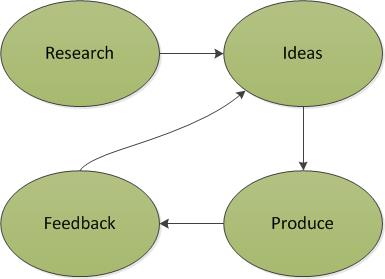
\includegraphics[width=0.6\textwidth]{metode.jpg}
  \caption [Method for constructing the \gls{quick} box.]{\textbf{Method for constructing the \gls{quick} box.}}
  \label{fig:metode}
\end{figure}


In addition to having knowledge about the company and its vision, it is important to gain an understanding of the technologies which are employed. This provides an opportunity for conducting further research and testing. After this initial theoretical learning process, we started looking at how Internet access can be provided to mesh networks. 

The theoretical insight gave us ideas as to how to expand the Mesh Potato's area of usage. We looked at specific scenarios in need of a communications system, and this brought forward the idea of creating a \gls{quick} box that could be applied for roll-out in different scenarios. The idea of the box is developed on the basis of previous work conducted by others. This work provided the foundation for our idea and development of the box. The prototype is provided with manuals describing how to connect an \gls{mp} to different uplinks. These manuals were tested on technical and "non-technical" people. The testing provided us with valuable feedback, which led to an improvement of the manuals. 

We also further developed the miscellaneous set-up descriptions provided by Village Telco. This became a big part of our assignment. Many of the existing descriptions are outdated and hard to understand, and also not valid for the second version of the Mesh Potato.



\section{Limitations}
Our main limitation was the amount of time we had available to finish our Masters thesis, since we only had 21 weeks at our disposal. When entering a new field it takes some time to understand the technology used. None of us have much experience with the different technologies used, and it took us some time to learn. Another limitation is money. We tried to get funding, from Engineers Without Borders, to visit an area recently affected by a natural disaster. Unfortunately they had no funding available at the moment. This restricted our research so it became more theoretical and less practical. We were therefore unable to test our solution and manuals on the actual end users. Instead we have conducted tests on people in our local community. These had both technical and "non-technical" backgrounds, all of them from the younger generation. In order to develop our solution further, it should be tested in real-world scenarios, as well as on a wider range of people. 


